\documentclass[a4,center,fleqn]{NAR}

% Enter dates of publication
\copyrightyear{2008}
\pubdate{31 July 2009}
\pubyear{2009}
\jvolume{37}
\jissue{12}

%\articlesubtype{This is the article type (optional)}

\begin{document}

\title{Helicobacter pylori Homology Database: the case of tryptophan}

\author{%
Markus Joppich\,$^{1,*}$,
Cindy?\,$^{2}$
Luisa Jimenez\,$^{3}$
and Ralf Zimmer\,$^1$%
\footnote{To whom correspondence should be addressed.
Tel: +49 89 2180 4045; Email: joppich@bio.ifi.lmu.de}}

\address{%
$^{1}$Affiliation of Corresponding Author
and
$^{2}$Affiliation of Both Co-Authors}
% Affiliation must include:
% Department name, institution name, full road and district address,
% state, Zip or postal code, country

\history{%
Received January 1, 2018;
Revised February 1, 2018;
Accepted March 1, 2018}

\maketitle

\begin{abstract}
	To study microorganisms it is necessary to evaluate phenotypes, which include biochemical and visual characteristic, and relation with its environment. The advance of sequencing technologies allow access to information about the organism's genome and how it is transcribed from multiple exemplars. The combination of genotype and phenotype result in a integral picture of a microorganism. However, large quantities of genomes are being submitted every day at a pace challenging the capacities of analysis for those studying an organism. To date most searches for homology genes / proteins are done with the objective of find unknown function based on homology to already known genes or proteins. This searches are important to estimate the function of unknown proteins or genes. However studies involving the analysis of homologous proteins across several clones from the same species are not being fully exploited at the moment; and if the researcher wants to take evaluate homlogous genes, it needs to rely on BLASTs or in a unanimous annotation of the genes of interest. The last is hardly achievable, leaving an tenuous and limited search through alignment. In order to show the advantages of genome / proteome information from several strains , we have developed a database using as model organism \textit {Helicobacter pylori}. With the use of this database we have found that strains from \textit{H. pylori} use tryptophan in proteins in a strain-specific way with potential changes in the function of membrane related and cation-binding proteins. We extended this analysis to other bacterial species adapting this database to their genome information, showing that it can be adapted to any microrganism of interest of which several genomes are complete.
\end{abstract}


\section{Introduction}

The idea that similar protein or gene sequences have a higher probability of fulfilling the same or similar function has been the foundation for searches based on alignments, being BLAST the most popular. Although similarity could mean analogous function, the lack of similitude does not exclude it. Alignments can help to discover the function of unknown genes or proteins under the premise that the function of a homologous sequence is already known, as variations of in sequences are considered part of the evolutionary process (reviewed by Pearson WR 2013).\\
Until 2015 there were genome sequences from 50 bacterial and 11 archaeal phyla available with a total of around 14000 (February 2015, NCBI) (Land M 2015). Today, over three years later,  this number has increase to a total of 133148 (March 15, 2018. NCBI Genome). The rate at which genomes are being published increases the possibility of finding a homologous gene or protein. At the same time, analysis of multiple genomes from different specimens (strains) belonging to same species allow to estimate normal variations of the organisms in ecosystems. However, this data growth rate challenges the ability to analyze it in a coherent manner based on already available information.\\	 


\begin{align*}
&\mathrm{Ascorbate} + \mathrm{EDTA} \cdot \mathrm{Fe}^{3+} \to
\hbox{Oxidized ascorbate}
\\
&\mathrm{EDTA} \cdot \mathrm{Fe}^{2+} + \mathrm{H}_2
\mathrm{O}_2 \to
\mathrm{EDTA} \cdot \mathrm{Fe}^{3+} + \cdot
\mathrm{OH} + \mathrm{OH}^-
\end{align*}

One of the many difficulties in the analysis of homologous proteins within one species is the variation of annotations in databases. Each submitted genome uses a different annotation for the genes/ proteins found in their data. Some are achieved through automated alignment and homology assignment. Other annotations are based on historic references made by the researchers at submission. One case are proteins components of the Type IV secretion System (T4SS). Bacterial species that present components for a T4SS, like Bordetella pertussis, Helicobacter pylori and Legionella pneumophila, have had their components described in different ways depending on the researcher submitting genomes,  or as a result of an automated homology search made. One example of the consequences for these variation in annotation of genomes is the L. pneumophila's component DotL (From the Dot/Icm T4SS). It can be found as across literature and genomes as DotL, IcmO, or referred as VirD4 homologue based on its resemblance to the first T4SS defined in Agrobacterium tumefasciens . However, if the text search is done using VirD4 in L. pneumophila, none of these proteins will appear. Instead the results will include LvhD4, VirD4 component, conjugal transfer protein TraG, hypothetical protein or Type IV secretory system conjugative DNA transfer family protein. 
% **************************************************************
% Keep this command to avoid text of first page running into the
% first page footnotes
\enlargethispage{-65.1pt}
% **************************************************************

This kind of variations in annotations makes the work with bacterial proteins names extremely difficult and frustrating. This case is not isolated: all other bacteria named above present the same challenges while working with T4SS, and although the variations in annotations of the T4SS could have been an exception, sadly it is more the rule for many of the annotations of genes in their genome.\\
Although there are several databases for homology search (HomoloGene from NCBI (Ref), OrtholugeDB (ref) and seac
In order to work with all homologous genes from one organism, the annotation's variations forces the use of sequence BLAST against the taxID of the species of interest, resulting in a list of proteins/genes with homologies to the query. This alignments can then be exported and used for analysis. Although functional is not the most efficient way to obtain several homologous genes from all strains sequenced.\\The database presented here is designed to eliminate the need of BLAST of each protein against its own database, and facilitate the comparison of genomic and proteomic data available in the EMBL genome database from different strains from the same organism.\\
To evaluate the effectiveness and usefulness of the database, we have chosen as model organism \textit{Helicobacter pylori}, an epsilon proteobacteria present in the human stomach and associated with gastric pathologies(ref). H. pylori is a natural competent bacterium, able to capture and integrate extracellular DNA into its genome. At the same time it present a high genetic variability between strains. The first strain sequenced from this organism was the strain 26695 (ref). Its open-reading frames (ORFs or Locus Tags) have been used for the definition of many  \textit{H. pylori} characteristic features, like the Cag Pathogenicity Island (Ref), the Outer Membrane Protein families (ref) and recently to describe the transcriptome of \textit{H. pylori}(Sharma et al). The strain J99 sequence followed and its locus tags have been used as synonym to describe proteins or genes. While these descriptions were sufficient to analyze single genes in the following years, the exponential growth of new genomes available and variations in annotations between strains makes it difficult to find the known homologue genes.
During experiments requiring semiquantitative analysis of western blot signals, the normalization of sample load for each bacterial strain in a polyacrylamide gel electrophoresis required the detection of proteins in a way compatible with further immunological analysis. The use of 2,2,2, trichloroethanol (TCE) with ultraviolet activation (ref) allowed the estimation of protein present in the gel and the use of the same samples for western blot analysis. The TCE allows fluorescent detection of tryptophan present in proteins at 305 nm without creating a crosslink of proteins with the acrylamide matrix. The imaging of tryptophan revealed that different strains presented variation in their patterns showing changes in tryptophan content in their proteins (Rojas et al, submitted) In order to find the homologous genes in two of the standard strains we were confronted with the need to identify the right homologous proteins in both genomes to quantify their tryptophan residues. This proved tedious and not really feasible if more strains would be analyzed. Therefore we created a database that allows the identification of homologous groups of proteins across different genomes independently of their annotations, and allows the introduction of transcriptome information if available for the organism. To show the biological reference using the database we show here that not only H. pylori uses tryptophan in an specific way, but ..... and ... as well, while other bacterial species like \textit{Escherichia coli} and \textit{Campylobacter pylori} restrict the variations in tryptophan residues.
Text \cite{2,3}.

Text \cite{4}.


\section{MATERIALS AND METHODS}

\subsection{Materials subsection one}

Text. Text. Text. Text. Text. Text. Text. Text. Text. Text. Text.
Text. Text. Text. Text. Text. Text. Text. Text. Text. Text. Text.
Text. Text. Text. Text. Text. Text. Text. Text. Text. Text. Text.
Text. Text. Text. Text. Text. Text. Text. Text. Text. Text. Text.
Text. Text. Text. Text. Text. Text. Text. Text. Text. Text. Text.
Text. Text. Text. Text. Text. Text. Text. Text. Text. Text. Text.
Text. Text. Text. Text. Text. Text. Text. Text. Text. Text. Text.
Text. Text. Text. Text. Text. Text. Text. Text. Text. Text. Text.
Text. Text. Text. Text. Text. Text. Text. Text. Text. Text. Text.
Text. Text. Text. Text. Text. Text. Text. Text. Text. Text. Text.
Text. Text. Text. Text. Text. Text. Text. Text. Text. Text. Text.
Text. Text. Text. Text. Text. Text. Text. Text. Text. Text. Text.
Text. Text. Text. Text. Text. Text. Text. Text. Text. Text. Text.
Text. Text. Text. Text. Text. Text. Text. Text. Text. Text. Text.
Text. Text. Text. Text. Text. Text. Text. Text. Text. Text. Text.
Text. Text. Text. Text. Text. Text. Text. Text. Text. Text. Text.
Text. Text. Text. Text. Text. Text. Text. Text. Text. Text. Text.
Text. Text. Text. Text. Text. Text. Text. Text. Text. Text. Text.
Text. Text. Text. Text. Text. Text. Text. Text. Text. Text. Text.
Text. Text. Text. Text. Text. Text. Text. Text. Text. Text. Text.
Text. Text. Text. Text. Text. Text. Text. Text. Text. Text. Text.
Text. Text. Text. Text. Text. Text. Text. Text. Text. Text. Text.
Text. Text. Text. Text. Text. Text. Text. Text. Text. Text. Text.
Text. Text. Text. Text. Text. Text. Text. Text. Text. Text.


\subsubsection{Materials subsubsection one.}

Text. Text. Text. Text. Text. Text. Text. Text. Text. Text. Text.
Text. Text. Text. Text. Text. Text. Text. Text. Text. Text. Text.
Text. Text. Text. Text:
\begin{align}
\mathrm{LD}^r = \frac{\mathrm{LD}}{A_\mathrm{iso}}
= 1.5 S \left( 3 \cos^2 \alpha_i - 1 \right)
\end{align}
Text. Text. Text. Text. Text. Text. Text. Text. Text. Text. Text.
Text. Text. Text. Text. Text. Text. Text. Text. Text. Text. Text.
Text. Text. Text. Text. Text. Text. Text. Text. Text. Text. Text.
Text. Text. Text. Text. Text. Text. Text. Text. Text. Text. Text.
Text. Text. Text. Text. Text. Text. Text. Text. Text. Text. Text.
Text. Text. Text. Text. Text. Text. Text. Text. Text. Text. Text.
Text. Text. Text. Text. Text. Text. Text. Text. Text. Text. Text.
Text. Text. Text. Text. Text. Text. Text. Text. Text. Text. Text.
Text. Text. Text. Text. Text. Text. Text. Text. Text. Text. Text.
Text. Text. Text. Text. Text. Text. Text. Text. Text. Text. Text.
Text. Text. Text. Text. Text. Text. Text. Text. Text. Text. Text.
Text. Text. Text. Text. Text. Text. Text. Text. Text. Text. Text.


\subsection{Materials subsection two}

Text. Text. Text. Text. Text. Text. Text. Text. Text. Text. Text.
Text. Text. Text. Text. Text. Text. Text. Text. Text. Text. Text.
Text. Text. Text. Text. Text. Text. Text
(see Figure \ref{NAR-fig1}).

Text. Text. Text. Text. Text. Text. Text. Text. Text. Text. Text.
Text. Text. Text. Text. Text. Text. Text. Text. Text. Text. Text.
Text. Text. Text. Text. Text. Text. Text. Text. Text. Text. Text.
Text. Text. Text. Text. Text. Text. Text. Text. Text. Text. Text.
Text. Text. Text. Text. Text. Text. Text.
\begin{equation*}
\mathrm{LD} \left( t \right) =
\sum\limits_i
a_i \exp \left( \frac{-t}{\tau_i} \right)
\end{equation*}
Text. Text. Text. Text. Text. Text. Text. Text. Text. Text. Text.
Text. Text. Text. Text. Text. Text. Text. Text. Text. Text. Text.
Text. Text. Text. Text. Text. Text. Text. Text. Text. Text. Text.
Text. Text. Text. Text. Text. Text. Text. Text. Text. Text. Text.
Text. Text. Text. Text. Text. Text. Text. Text. Text. Text. Text.
Text. Text. Text. Text. Text. Text. Text. Text. Text. Text. Text.
Text. Text. Text. Text.

\begin{figure}[t]
\begin{center}
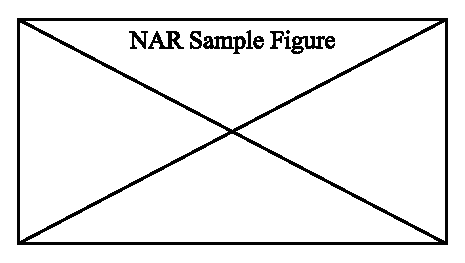
\includegraphics{NAR-fig1.eps}
\end{center}
\caption{Caption for figure within column.}
\label{NAR-fig1}
\end{figure}


\section{RESULTS}

\subsection{Results subsection one}

Text. Text. Text. Text. Text. Text. Text. Text. Text. Text. Text.
Text. Text. Text. Text. Text. Text. Text. Text. Text. Text. Text.
Text. Text. Text. Text. Text. Text. Text. Text. Text. Text. Text.
Text. Text. Text. Text. Text. Text. Text. Text. Text. Text. Text.
Text. Text. Text. Text. Text. Text. Text. Text. Text. Text. Text.
Text. Text. Text. Text. Text. Text. Text. Text. Text. Text. Text.
Text. Text. Text. Text. Text. Text. Text. Text. Text. Text. Text.
Text. Text. Text. Text. Text. Text. Text. Text. Text. Text. Text.
Text. Text. Text. Text. Text. Text. Text. Text. Text. Text. Text.
Text. Text. Text. Text. Text. Text. Text. Text. Text. Text. Text.
Text. Text. Text. Text. Text. Text. Text. Text. Text. Text. Text.
Text. Text. Text. Text. Text. Text. Text. Text. Text.

\begin{table}[b]
\tableparts{%
\caption{This is a table caption}
\label{table:01}%
}{%
\begin{tabular*}{\columnwidth}{@{}lllll@{}}
\toprule
Col. head 1 & Col. head 2 & Col. head 3 & Col. head 4 & Col. head 5
\\
& (\%) & (s$^{-1}$) & (\%) & (s$^{-1}$)
\\
\colrule
Row 1 & Row 1 & Row 1 & -- & --
\\
Row 2 & Row 2 & Row 2 & Row 2 & Row 2
\\
\botrule
\end{tabular*}%
}
{This is a table footnote}
\end{table}


\subsection{Results subsection two}

Text.  Text. Text. Text. Text. Text. Text. Text. Text. Text. Text.
Text. Text. Text. Text. Text. Text. Text. Text. Text. Text. Text.
Text (see Table \ref{table:01}).

Text. Text. Text. Text. Text. Text.
Text. Text. Text. Text. Text. Text. Text. Text. Text. Text. Text.
Text. Text. Text. Text. Text. Text. Text. Text. Text.
Text (see Figure \ref{NAR-fig2}a).

Text. Text. Text. Text. Text.
Text. Text. Text. Text. Text. Text. Text. Text. Text. Text. Text.
Text. Text. Text. Text. Text. Text. Text. Text. Text. Text. Text.
Text. Text. Text. Text. Text. Text. Text. Text. Text. Text. Text.
Text. Text. Text. Text. Text. Text. Text. Text. Text. Text. Text.
Text. Text. Text. Text. Text. Text. Text. Text. Text. Text. Text.
Text. Text. Text. Text. Text. Text. Text. Text. Text. Text. Text.
Text. Text. Text. Text. Text. Text. Text. Text. Text. Text. Text.
Text. Text. Text. Text. Text. Text. Text. Text. Text. Text. Text.
Text. Text. Text. Text. Text. Text. Text. Text. Text. Text. Text.
Text. Text. Text. Text. Text. Text. Text. Text. Text. Text. Text.
Text. Text. Text. Text. Text. Text. Text. Text. Text. Text.

\begin{figure*}[t]
\begin{center}
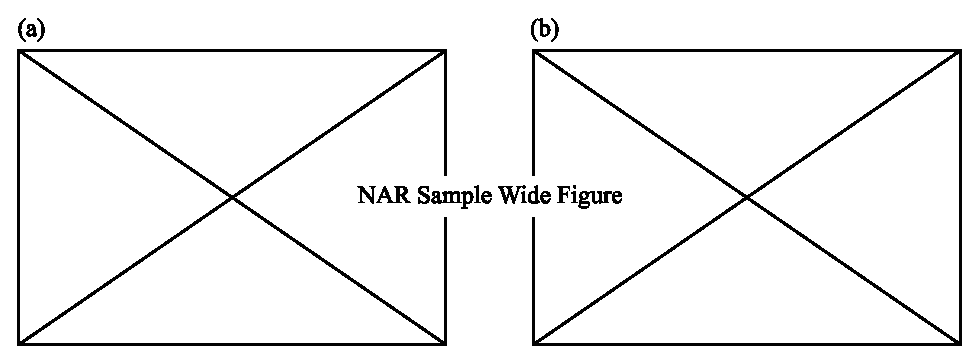
\includegraphics{NAR-fig2.eps}
\end{center}
\caption{Caption for wide figure over two columns.
\textbf{(a)} Left figure.
\textbf{(b)} Right figure (see (a)).
}
\label{NAR-fig2}
\end{figure*}


\subsection{Results subsection three}

Text. Text. Text. Text. Text. Text. Text. Text. Text. Text. Text.
Text. Text. Text. Text. Text. Text. Text. Text. Text. Text. Text.
Text. Text. Text. Text. Text. Text. Text. Text. Text. Text. Text.
Text. Text. Text. Text. Text. Text. Text. Text. Text. Text. Text.
Text. Text. Text. Text. Text. Text. Text. Text. Text. Text. Text.
Text. Text. Text. Text. Text. Text. Text. Text. Text. Text. Text.
Text. Text. Text. Text. Text. Text. Text. Text. Text. Text. Text.
Text. Text. Text. Text. Text. Text. Text. Text. Text. Text. Text.
Text. Text. Text. Text. Text. Text. Text. Text. Text. Text. Text.
Text. Text. Text. Text. Text. Text. Text. Text. Text. Text. Text.
Text. Text. Text.


\section{DISCUSSION}

\subsection{Discussion subsection one}

Text. Text. Text. Text. Text. Text. Text. Text. Text. Text. Text.
Text. Text. Text. Text. Text. Text. Text. Text. Text. Text. Text.
Text. Text. Text. Text. Text. Text. Text. Text. Text. Text. Text.
Text. Text. Text. Text. Text. Text. Text. Text. Text. Text. Text.
Text. Text. Text. Text. Text. Text. Text. Text. Text. Text. Text.
Text. Text. Text. Text. Text. Text. Text. Text. Text. Text. Text.
Text. Text. Text. Text. Text. Text. Text. Text. Text. Text. Text.
Text. Text. Text. Text. Text. Text. Text. Text. Text. Text. Text.
Text. Text. Text. Text. Text. Text. Text. Text. Text. Text. Text.
Text. Text. Text. Text. Text. Text. Text. Text. Text. Text. Text.
Text. Text. Text. Text. Text. Text. Text. Text. Text. Text. Text.
Text. Text. Text. Text. Text. Text. Text. Text. Text. Text. Text.
Text. Text. Text. Text. Text. Text. Text. Text. Text. Text. Text.
Text. Text. Text. Text. Text. Text. Text. Text. Text. Text. Text.
Text. Text. Text. Text. Text. Text. Text. Text. Text. Text. Text.
Text. Text. Text. Text. Text. Text. Text. Text. Text. Text. Text.
Text. Text. Text. Text. Text. Text. Text. Text. Text. Text. Text.
Text. Text. Text. Text. Text. Text. Text. Text. Text. Text. Text.
Text. Text. Text. Text. Text. Text. Text. Text. Text. Text. Text.
Text. Text. Text. Text. Text. Text. Text. Text. Text. Text. Text.
Text. Text. Text. Text. Text. Text.


\subsection{Discussion subsection two}

Text. Text. Text. Text. Text. Text. Text. Text. Text. Text. Text.
Text. Text. Text. Text. Text. Text. Text. Text. Text. Text. Text.
Text. Text. Text. Text. Text. Text. Text. Text. Text. Text. Text.
Text. Text. Text. Text. Text. Text. Text. Text. Text. Text. Text.
Text. Text. Text. Text. Text. Text. Text. Text. Text. Text. Text.
Text. Text. Text. Text. Text. Text. Text. Text. Text. Text. Text.
Text. Text. Text. Text. Text. Text. Text. Text. Text. Text. Text.
Text. Text. Text. Text. Text. Text. Text. Text. Text. Text. Text.
Text. Text. Text. Text. Text. Text. Text. Text. Text. Text. Text.
Text. Text. Text. Text. Text. Text. Text. Text. Text. Text. Text.
Text.

Text. Text. Text. Text. Text. Text. Text. Text. Text. Text. Text.
Text. Text. Text. Text. Text. Text. Text. Text. Text. Text. Text.
Text. Text. Text. Text. Text. Text. Text. Text. Text. Text. Text.
Text. Text. Text. Text. Text. Text. Text. Text. Text. Text. Text.
Text. Text. Text. Text. Text. Text. Text. Text. Text. Text. Text.
Text. Text. Text. Text. Text. Text. Text. Text. Text. Text. Text.
Text. Text. Text. Text. Text. Text. Text. Text. Text. Text. Text.
Text. Text. Text. Text. Text. Text. Text. Text. Text. Text. Text.
Text. Text. Text. Text. Text. Text. Text. Text. Text. Text. Text.
Text. Text. Text. Text. Text. Text. Text. Text. Text. Text. Text.
Text. Text. Text. Text. Text. Text. Text. Text. Text. Text.


\subsection{Discussion subsection three}

Text. Text. Text. Text. Text. Text. Text. Text. Text. Text. Text.
Text. Text. Text. Text. Text. Text. Text. Text. Text. Text. Text.
Text. Text. Text. Text. Text. Text. Text. Text. Text. Text. Text.
Text. Text. Text. Text. Text. Text. Text. Text. Text. Text. Text.
Text. Text. Text. Text. Text. Text. Text. Text. Text. Text. Text.
Text. Text. Text. Text. Text. Text. Text. Text. Text. Text. Text.
Text. Text. Text. Text. Text. Text. Text. Text. Text. Text. Text.
Text. Text. Text. Text. Text. Text. Text. Text. Text. Text. Text.
Text. Text. Text. Text. Text. Text. Text. Text. Text. Text. Text.
Text. Text. Text. Text. Text. Text. Text. Text. Text. Text. Text.
Text. Text. Text. Text. Text. Text. Text. Text. Text.

Text. Text. Text. Text. Text. Text. Text. Text. Text. Text. Text.
Text. Text. Text. Text. Text. Text. Text. Text. Text. Text. Text.
Text. Text. Text. Text. Text. Text. Text. Text. Text. Text. Text.
Text. Text. Text. Text. Text. Text. Text. Text. Text. Text. Text.
Text. Text. Text. Text. Text. Text. Text. Text. Text. Text. Text.
Text. Text. Text. Text. Text. Text. Text. Text. Text. Text. Text.
Text. Text. Text. Text. Text. Text. Text. Text. Text. Text. Text.
Text. Text. Text. Text. Text. Text. Text.

Text. Text. Text. Text. Text. Text. Text. Text. Text. Text. Text.
Text. Text. Text. Text. Text. Text. Text. Text. Text. Text. Text.
Text. Text. Text. Text. Text. Text. Text. Text. Text. Text. Text.
Text. Text. Text. Text. Text. Text. Text. Text. Text. Text. Text.
Text. Text. Text. Text. Text. Text. Text. Text. Text. Text. Text.
Text. Text. Text. Text. Text. Text. Text. Text. Text. Text. Text.
Text. Text. Text. Text. Text. Text. Text. Text. Text. Text. Text.
Text. Text. Text. Text. Text. Text. Text.


\section{CONCLUSION}

Text. Text. Text. Text. Text. Text. Text. Text. Text. Text. Text.
Text. Text. Text. Text. Text. Text. Text. Text. Text. Text. Text.
Text. Text. Text. Text. Text. Text. Text. Text. Text. Text. Text.
Text. Text. Text. Text. Text. Text. Text. Text. Text. Text. Text.
Text. Text. Text. Text. Text. Text. Text. Text. Text. Text. Text.
Text. Text. Text. Text. Text. Text. Text. Text. Text. Text. Text.
Text. Text. Text. Text. Text. Text. Text. Text. Text. Text. Text.
Text. Text. Text. Text. Text. Text. Text. Text. Text. Text. Text.
Text. Text. Text. Text. Text. Text. Text. Text. Text. Text. Text.
Text. Text. Text.


\section{ACKNOWLEDGEMENTS}

Text. Text. Text. Text. Text. Text. Text. Text. Text. Text. Text.
Text. Text. Text. Text.


\subsubsection{Conflict of interest statement.} None declared.
\newpage


\begin{thebibliography}{4}

% Format for article
\bibitem{1}
Author,A.B. and Author,C. (1992)
Article title.
\textit{Abbreviated Journal Name}, \textbf{5}, 300--330.

% Format for book
\bibitem{2}
Author,D., Author,E.F. and Author,G. (1995)
\textit{Book Title}.
Publisher Name, Publisher Address.

% Format for chapter in book
\bibitem{3}
Author,H. and Author,I. (2005)
Chapter title.
In
Editor,A. and Editor,B. (eds),
\textit{Book Title},
Publisher Name, Publisher Address,
pp.\ 60--80.

% Another article
\bibitem{4}
Author,Y. and Author,Z. (2002)
Article title.
\textit{Abbreviated Journal Name}, \textbf{53}, 500--520.

\end{thebibliography}

\end{document}
